\section{V11}
\subsection{Subroutinen}
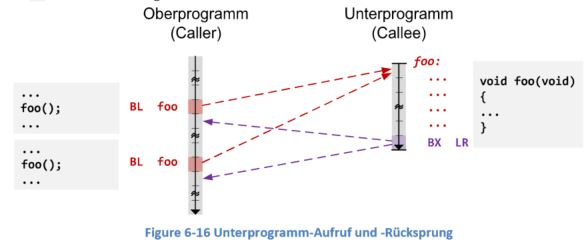
\includegraphics[width=0.8\linewidth]{images/subroutinen} 

\subsection{Architecure Producer Call Standart (AAPCS)}
\subsubsection{Regeln}
\begin{itemize}
    \item Bei Funktionsaufrufen werden die Register \textbf{R0-R3} als \textbf{Parameter} an eine C-Funktion verwendet
    \item Die Funktionen müssen die Inhalte der Register \textbf{R4-R11}(falls benutzt) während der Ausführung sichern, um sie am Ende wieder rekonstruieren
    \item Der \textbf{Rückgabewert} einer Subroutine (8-bit, 16-bit,32-bit) wird in den \textbf{Registern R0} übertragen. Handelt es sich um einen 64-bit Rückgabewert, so sind die unteren 32-bit im Register R0 und die oberen 32-bit im Register R1 übertragen
    \item Mit PUSH und POP wird immer eine \textbf{gerade Anzahl von Registern auf dem Stack} gelegt bzw. vom Stack eine \textbf{8-byte Alignment} auf dem Stack einzuhalten
\end{itemize}